%\documentclass[wsdraft]{ws-procs11x85}

\documentclass{ws-procs11x85}
\usepackage{ws-procs-thm}           % comment this line when `amsthm / theorem / ntheorem` package is used
\usepackage{multirow}
\usepackage{tabularx}
\newcommand{\etal}{\textit{et al}.}

\begin{document}

\title{Ultra-Fast and Scalable Quantification Pipeline of Transcript Abundances from Next Generation Sequencing Data}

\author{Hyun-Hwan Jeong$^{1,2}$, Hari Krishna Yalamanchili$^{1,2}$, and Zhandong Liu$^{2,3,\dag}$}

\address{$^{1}$Department of Molecular and Human Genetics, Baylor College of Medicine,\\
$^{2}$Jan and Dan Duncan Neurological Research Institute, Texas Children’s Hospital,\\
$^{3}$Department of Pediatrics, Baylor College of Medicine,\\
Houston, Texas 77030, USA\\
$^{\dag}$E-mail: zhandonl@bcm.edu}

\begin{abstract}
TODO: Writing abstract...
\end{abstract}

\keywords{Transposon Element;Alignment Free Quantification;Next Generation Sequencing}

% required
\copyrightinfo{\copyright\ 2017 The Authors. Open Access chapter published by World Scientific Publishing Company and distributed under the terms of the Creative Commons Attribution Non-Commercial (CC BY-NC) 4.0 License.}

% required
\bodymatter

\section{Introduction}\label{aba:intro}

\begin{itemize}
\item Importance of TE transcriptome quantification
\item Introductory of various tool
	\begin{itemize}
    \item However, it is very slow - need BAM
    \item Or it needs a customization
    \end{itemize}
\item Fast quantification tools are rising
\item We have made a pipeline
\end{itemize}


\section{Methods}


The proposed pipeline consists of three parts: Transposon element library preparation, quantification, and statistical analysis. Fig. \ref{aba:fig1}. introduce how this proposed pipeline works.
The entire source codes and executable scripts are available at \url{https://github.com/hyunhwaj/SalmonTE}. We describe details of the pipeline in this section. 
% Is it better to say "three parts" than "two parts?"

\begin{figure}[!ht]
\centerline{
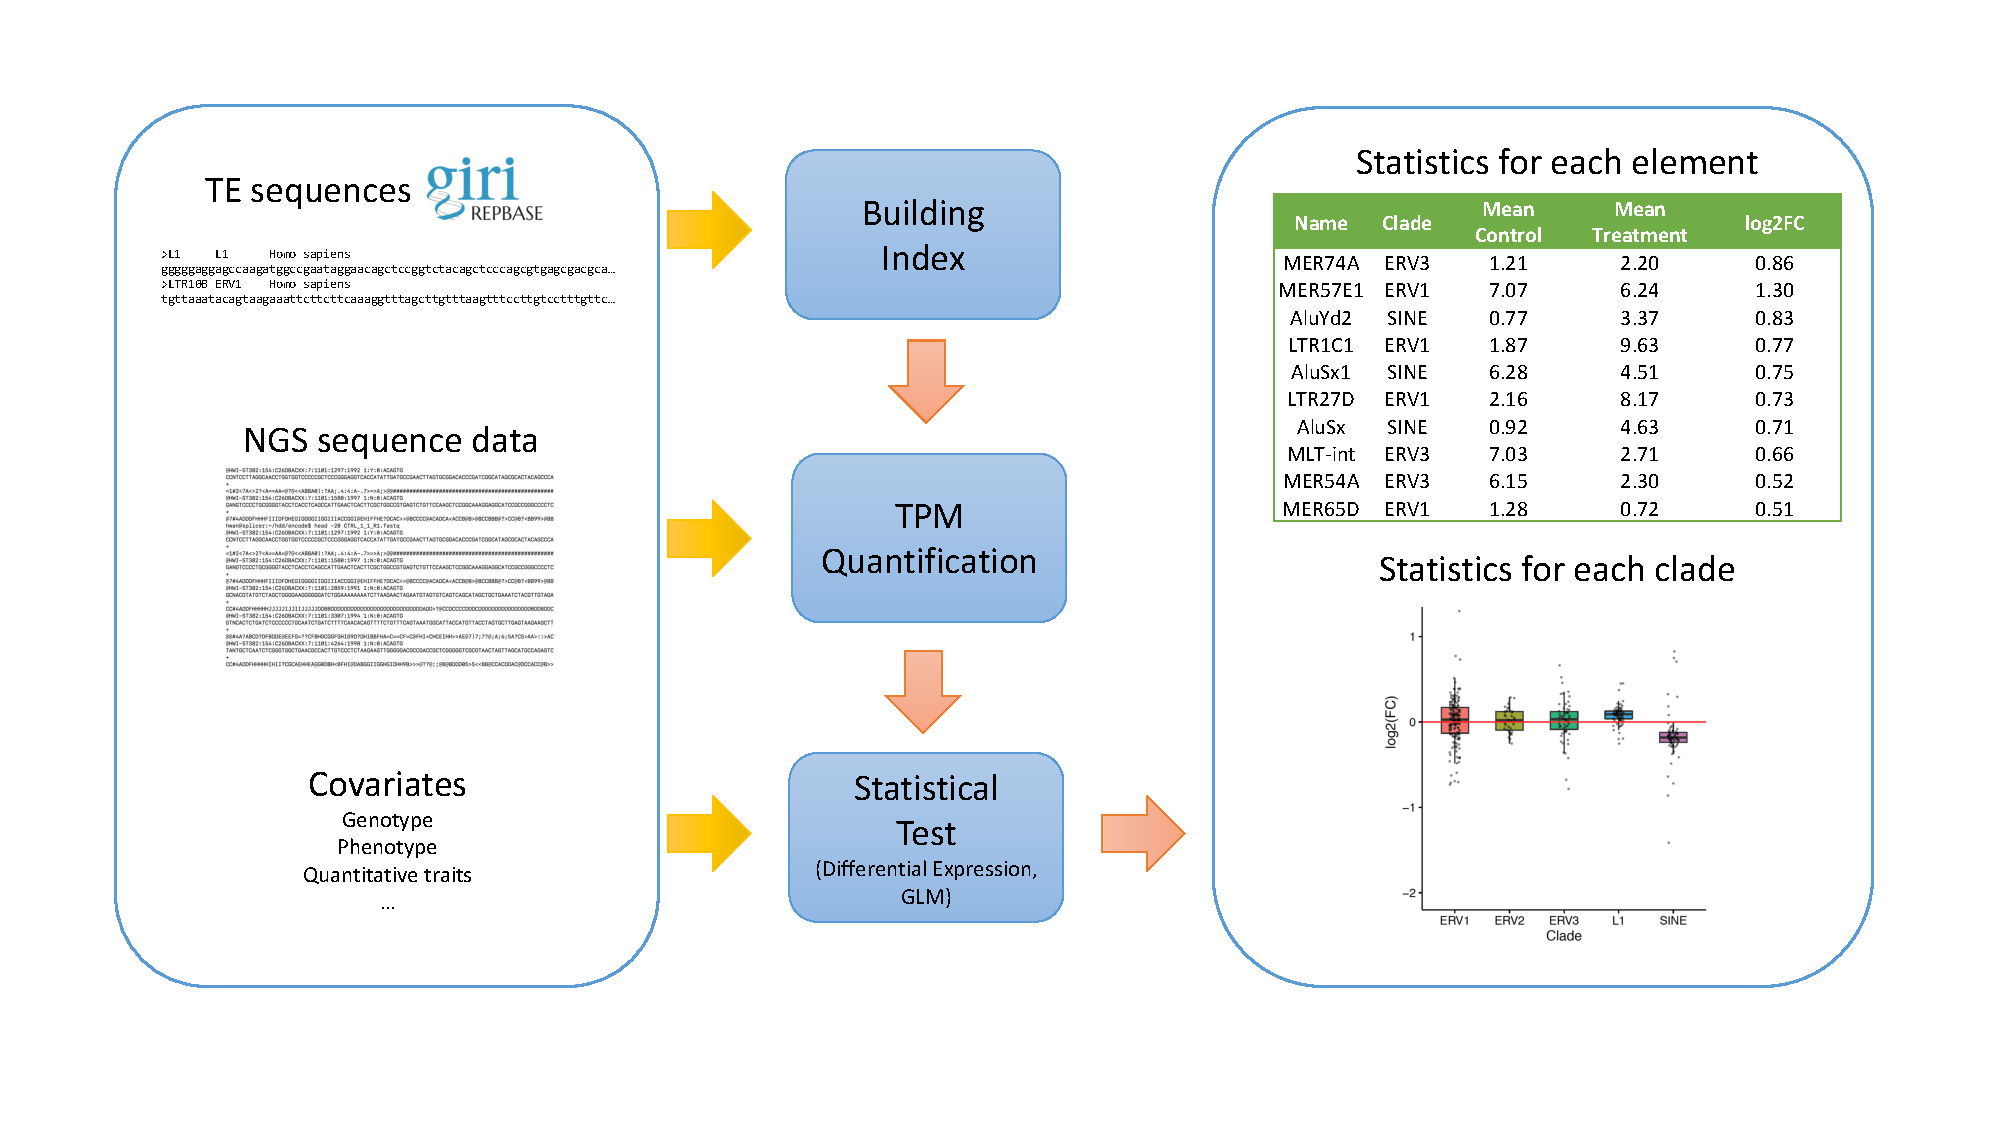
\includegraphics[width=16cm]{fig1.pdf}
}
\caption{An illustration of the SalmonTE pipeline}
\label{aba:fig1}
\end{figure}

\subsection{Transposon Element Library Preparation}

We collected the consensus cDNA sequence library of TEs for \textit{Homo Sapiens} and \textit{Drosophila Melanogaster} from Repbase  
(version 22.06)\cite{repbase}. We did not include sequences of simple repeats and multicopy genes, and DNA transposons (which replicate without an RNA intermediate). Once we collected the library, we manually curated clades of each TE, based on the annotation of Repbase. As a result, we have ? TEs for \textit{Homo Sapiens} and ? TEs for \textit{Drosophila Melanogaster}.
% need to add a table to summarize, will put the information

\subsection{Salmon quantification algorithm}

We deploy Salmon\cite{patro2017salmon} to quantify the transposon elements abundance from given RNA-seq reads files. Salmon enables a fast and accurate quantification of transcript expression from RNA-seq reads with quasi-mapping, a variant of stochastic, collapsed variational Bayesian inference(in the online phase), and Expectation Maximization (EM) algorithm (in the offline phase)
\cite{patro2017salmon,srivastava2016rapmap,bishop2006pattern,foulds2013stochastic}. 
To facilitate running this step easier, and to enable parallel processing for multiple RNA-seq reads files, we adopted Snakemake workflow system and wrote a script of the execution rule for the system.\cite{koster2012snakemake}
% Still completing pipeline, and it will out to github and our website.

\subsection{Statistical tests}

With the covariates data for given samples in the experiments, 
we perform statistical analysis between quantified TE abundance between the quantified TE expressions from Salmon and the covariate as the last step of the pipeline. Differential analysis using DEseq2 can perform for binary covariates such as binary genotype, phenotype and gender \cite{love2014moderated}, and 
we can apply General Linear Model (GLM) for quantitative covariate such as disease pathology score and age. \cite{johnston1980multivariate}. The analysis will make two different outputs. The first one is the statistics for each TE, and the second one is the summary of the statistics for each clade. The output files are provided as various file formats such as tab-separated values file (TSV), XML spreadsheet file format (XLS, XLSX), R object file (Rdata), and Portable Document Format (PDF) file.

\section{Results}

In the paper of TEtranscripts, they demonstrated that TEtranscripts is the best method among the published methods 
in terms of recovery accuracy of TE and running time for both cases of synthetic dataset and published data. 
Therefore, we only compare our pipeline with TEtranscripts. 
Ohthani \etal's RNA-seq data, which were used in the TEtranscripts paper, were also used to compare between 
our proposed pipeline and TEtranscripts. \cite{ohtani2013dmgtsf1}  

\subsection{Performance Benchmarking of SalmonTE}

\begin{table}[h]
\tbl{Performance comparison between SalmonTE and TEtranscripts}
{\begin{tabular}{l|ll}
\hline
Dataset                          & Piwi KD    & Encode TARDBP \\ \hline
Total number of samples          & 2          & 4             \\ 
RNA-seq file type                & Single end & Paired ends  \\ 
Total number of reads            & 90,411,467 & 309,701,182   \\ \hline
SalmonTE runtime (hh:mm:ss)      & 0:05:33    & 0:17:13       \\
TEtranscripts runtime (hh:mm:ss) & 1:45:26    & 7:49:40       \\
Speedup                          & 19.00x     & 27.28x        \\ \hline
\end{tabular}}\label{aba:table1}
\end{table}

\subsection{Quantification}
\begin{figure}[h]
\centerline{
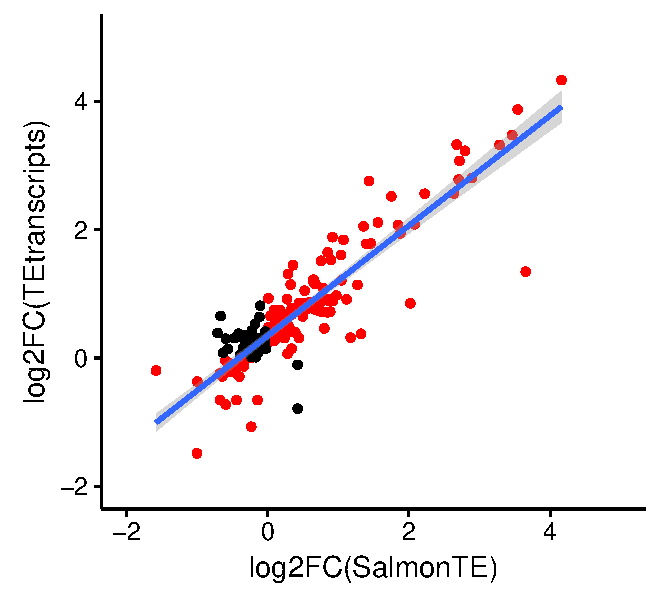
\includegraphics[width=11cm]{figure_corr_FC}
}
\caption{Correlation of $log_{2}FC$ ($\frac{Piwi}{Control}$) for each transposon element between SalmonTE and TEtranscripts. Red points represents points shows same sign of estimated $log_{2}FC$ from SalmonTE and TEtranscripts.}
\label{aba:fig2}
\end{figure}

\begin{figure}[h]
\centerline{
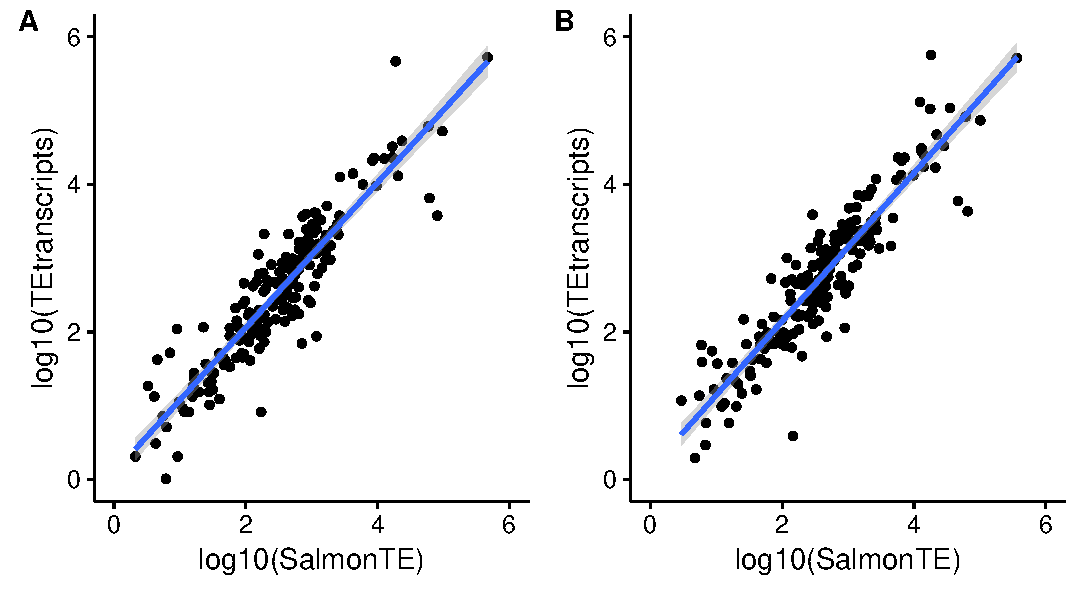
\includegraphics[width=16cm]{figure_corr_count}
}
\caption{Sample correlation of count for each transposon element between SalmonTE and TEtranscripts}
\label{aba:fig3}
\end{figure}

%\begin{table}[h]
%\tbl{Sample correlation of count for each transposon element between SalmonTE and TEtranscripts}
%{\begin{tabular}{cccccc}
%\cline{3-6}
%                               &         & \multicolumn{2}{c}{SalmonTE} & \multicolumn{2}{c}{TETranscripts} \\ \cline{3-6} 
%                               &         & Control        & Piwi        & Control           & Piwi          \\ \hline
%\multirow{2}{*}{SalmonTE}      & Control & 1.00           & 0.93        & 0.91              & 0.86          \\ \cline{2-6} 
%                               & Piwi    &                & 1.00        & 0.87              & 0.92          \\ \hline
%\multirow{2}{*}{TETranscripts} & Control &                &             & 1.00              & 0.95          \\ \cline{2-6} 
%                               & Piwi    &                &             &                   & 1.00          \\ \hline
%\end{tabular}}\label{aba:table1}
%\end{table}


\begin{figure}[h]
\centerline{
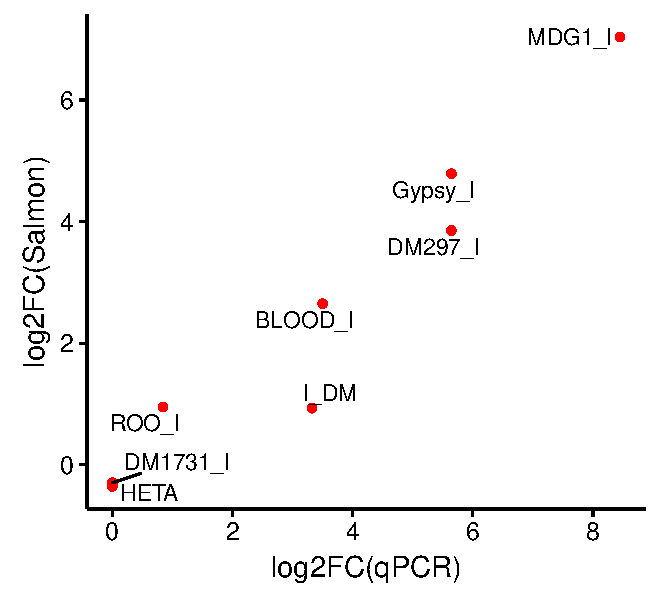
\includegraphics[width=15cm]{supp_fig3_corr}
}
\caption{Comparison between SalmonTE and RT-qPCR}
\label{aba:fig4}
\end{figure}


\subsection{Demonstration on human cell-line TARDBP data}

\begin{table}[h]
\tbl{23 Differentially expressed transposon elements in the ENCODE TARDBP data}{
\begin{tabular*}{.5\textwidth}{@{\extracolsep{\fill}}ccc}
\hline
Name & Clade & log2FC\\
\hline
MER74A & ERV3 & 1.68\\
MER57E1 & ERV1 & 1.30\\
AluYd2 & SINE & 0.83\\
LTR1C1 & ERV1 & 0.77\\
AluSx1 & SINE & 0.75\\
LTR27D & ERV1 & 0.73\\
AluSx & SINE & 0.71\\
MLT-int & ERV3 & 0.66\\
MER54A & ERV3 & 0.52\\
MER65D & ERV1 & 0.51\\
LTR28 & ERV1 & -0.59\\
LTR1F & ERV1 & -0.63\\
FLAM & SINE & -0.64\\
MER21 & ERV3 & -0.68\\
MER101 & ERV1 & -0.69\\
LTR26B & ERV1 & -0.70\\
MER83C & ERV1 & -0.71\\
AluJo & SINE & -0.72\\
LTR06 & ERV1 & -0.73\\
MLT2D & ERV3 & -0.78\\
AluYf5 & SINE & -0.86\\
AluYd3 & SINE & -1.41\\
THER2 & SINE & -2.03\\ \hline
\end{tabular*}}\label{aba:table2}
\end{table}


\begin{figure}[h]
\centerline{
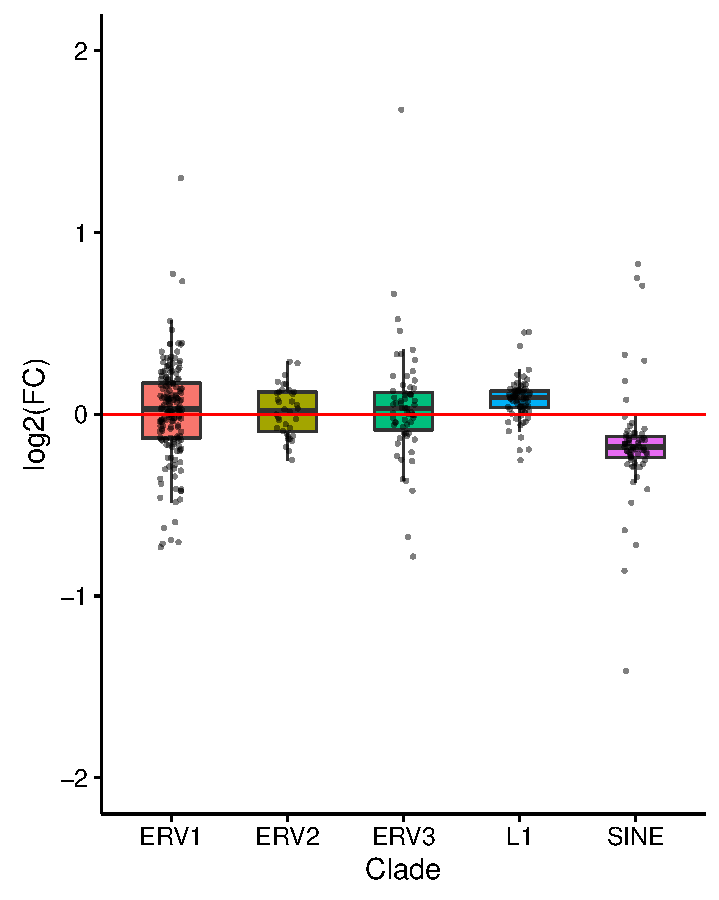
\includegraphics[width=13cm]{boxplot-clade-k562}
}
\caption{An boxplot of $log_{2}FC$ for each clade in the ENCODE TARDBP data}
\label{aba:fig5}
\end{figure}


\bibliographystyle{ws-procs11x85}
\bibliography{ws-pro-sample}

\end{document}